\section{Model fizyczny bazy danych}

Na Rysunku \ref{fig:diagram} znajduje się schemat (diagram tabel) wygenerowanej przez skrypt:
\\
\href{run:skrypt_tworzacy_obiekty_w_bazie_danych.sql}{\texttt{skrypt\_tworzacy\_obiekty\_w\_bazie\_danych.sql}}.

\begin{figure}[h]
	\centering
	\caption{Diagram tabel wygenerowanej bazy danych}
    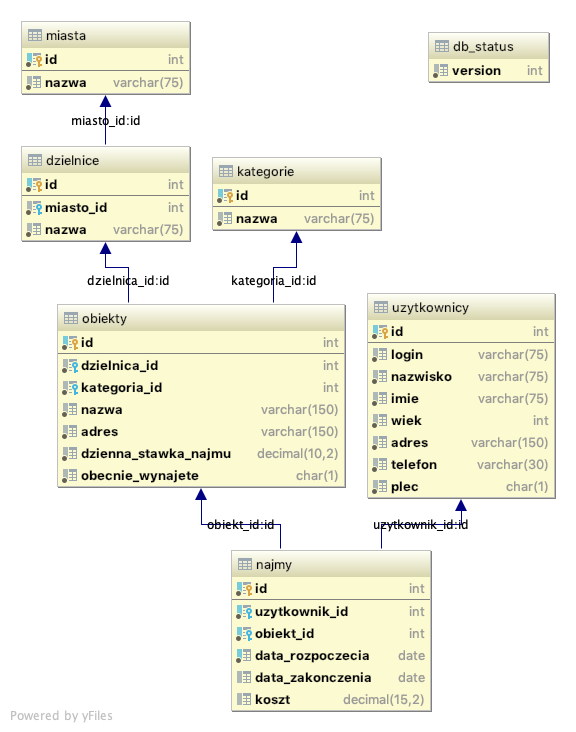
\includegraphics[width=0.5\textwidth]{diagram}
	\label{fig:diagram}
\end{figure}